\documentclass[9pt, dvipsnames,compress,aspectratio=169]{beamer}
\usepackage{winthrop-slides}
\addbibresource{biblio.bib}
\date{\today}

\title[AD Dynamics]{Modeling the Dynamics of Alzheimer's Disease} %still need a better title
\subtitle{Winthrop University}
\author[Loveless, Nix, Stokes]{Landon Loveless \and Garrett Nix \and Steven Stokes}
\institute[]{
\includegraphics[height=1cm]{img/WU-Logo2.pdf}}

\begin{document}
\begin{frame}[plain]
    \titlepage
\end{frame}
\begin{frame}{Table of Contents}
    \tableofcontents
\end{frame}

\section{Introduction} %Section start
\subsection{A Brief Synopsis of Alzheimer's Disease}

\begin{frame}{What Alzheimer's Disease Is}
    Alzheimer's Disease (AD) is a neurodegenerative disease characterized by many complex interactions that affect over 50 million people worldwide.
    Many different aspects of the disease are anticipated, but it is not yet known how these factors interact \cite{maji2025mathematical}.

    \begin{figure}
        \centering
        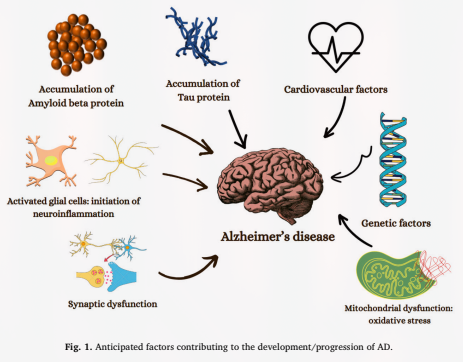
\includegraphics[width=0.3\textwidth]{img/ad_diagram_of_factors.png}
        \caption{Various factors of AD from the literature}
    \end{figure}
\end{frame}

\begin{frame}{Hypotheses Galore}
    Various hypotheses have been proposed in order to understand the underlying mechanisms of AD; where the leading hypothesis for many years has been the \textit{Amyloid Cascade Hypothesis}. 
    However, there has been increasing support in the notion that it is insufficient in giving an effective description and treatment towards AD: 
    many recent trials in studying the effect of $A_\beta$ blockers are failing to have meaningful effects. \cite{kepp2023amyloid}.
    This motivates the need for pursuing new avenues of treatment.

    \begin{figure}
        \centering
        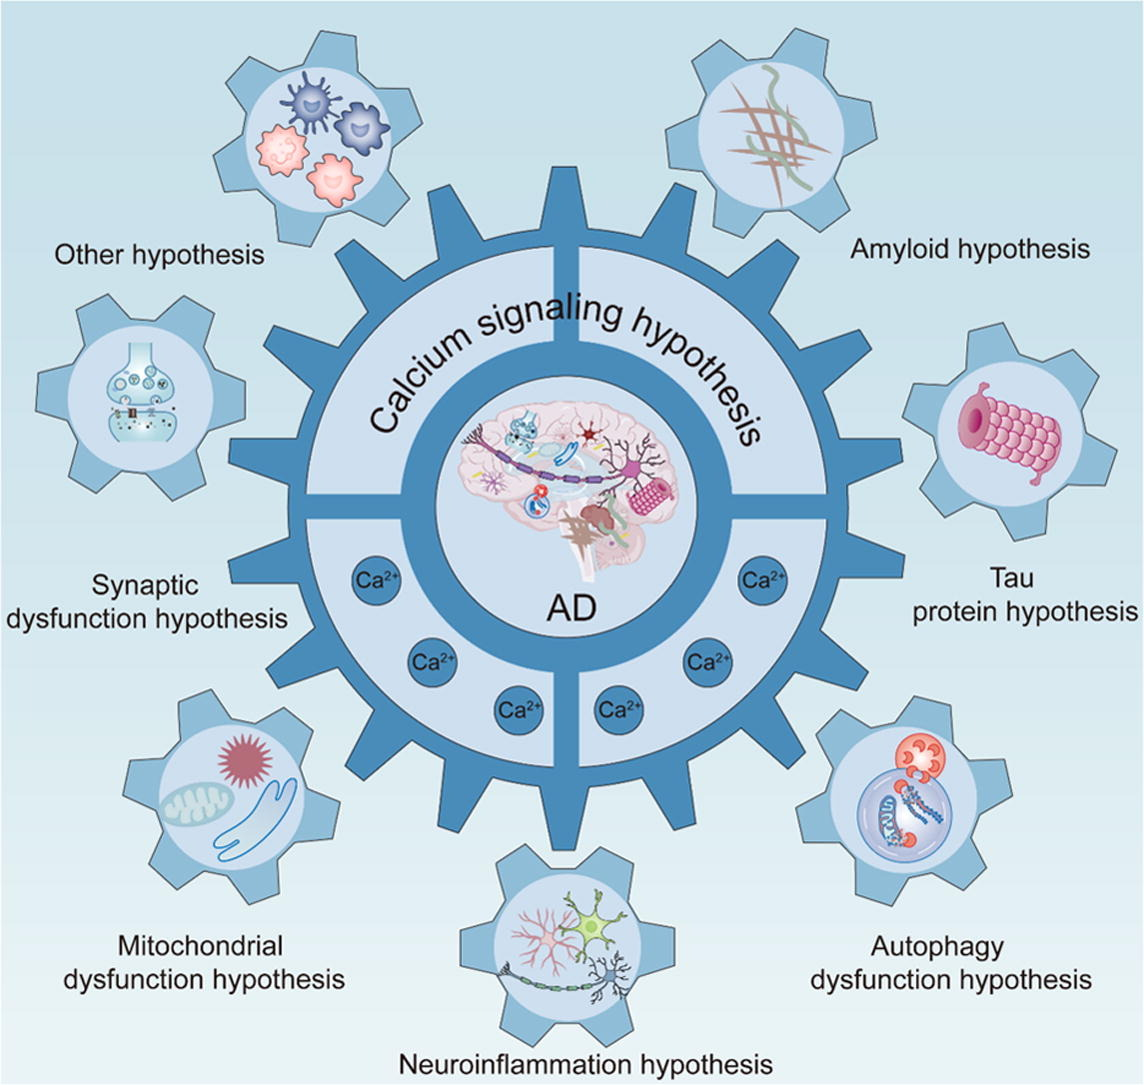
\includegraphics[width=0.3\textwidth]{img/new_hypotheses_galore.jpg}
        \caption{Various factors of AD from the literature}
    \end{figure}
\end{frame}
\section{Formation of Proposed Model}

\begin{frame}{Formation of a Newly Proposed Model}
    In order to understand these factors and subsequently the behavior of AD, many systems of ordinary differential equations (ODEs) have been proposed related to these hypotheses; but, a few are highlighted in regard to creating a newly proposed dynamical system:
    \begin{itemize}
        \item Observing the dynamics between $A_\beta$ and $Ca ^{2+}$ \cite{pal2025nonequilibrium}.
        \item Using causal models observing factors of genetic, non-amyloid dependent, and biomarker cascades \cite{petrella2019computational}.
    \end{itemize}
\end{frame}

\begin{frame}{The Proposed Model}
    Due to the feedback loop created by $A_\beta$ and $Ca ^{2+}$, along with the interaction between the hyperphosphorylation of $\tau$-protein caused by $A_\beta$, a proposed causal model is described by the following system of ODEs:
    \begin{eqnarray}
        \frac{dA _{\beta}}{dt}&=&a _{1}+\underbrace{a _{2}\frac{Ca}{Ca+\sigma}}_{\text{Michaelis-Menton}}- k_1 A _{\beta} - u_1 A_\beta\\
        \frac{dCa}{dt}&=& b _{1}+b _{2}A _{\beta}- k_2 Ca - u_2 Ca\\
        \frac{d \tau}{dt}&=&c _{1}+\underbrace{c _{2}A _{\beta}+c _{3}Ca}_{\text{$A_\beta$, Ca $^{2+}$ interaction}}- k_3 \tau - u_3 \tau\\
        \frac{dN}{dt}&=&d _{1}+d _{2}\tau-k _{4}N\\
        \frac{dC}{dt}&=&e _{1}+e _{2}NR + e _{3}\tau - k_5 C,
    \end{eqnarray}
    where $k_n$ is the natural removal rate and $u_n$ is the treatment parameter.
\end{frame}

\subsection{Stability Analysis}
\begin{frame}{On Invariance and Boundedness}

    The system can be shown to be \textit{positively invariant}. This is shown by 
    \begin{equation*}
        \left.\frac{dA _{\beta}}{dt}\right|_{A _{\beta}=0}, \left.\frac{dCa}{dt}\right|_{Ca=0}, \left.\frac{d\tau}{dt}\right|_{\tau=0},\left.\frac{dN}{dt}\right|_{N=0},\left.\frac{dC}{dt}\right|_{C=0} \geq 0.
    \end{equation*}
    Since the model follows biological scenarios, non-negative parameter choices mean that each compartment is non-negative, and thus the non-negative orthant is invariant. \bigskip

    The system can also be shown to be \textit{bounded} by
    \begin{eqnarray*}
        \frac{d A_\beta}{dt} = a _{1}+a _{2}\frac{Ca}{Ca+\sigma} -r _{1}A _{\beta} &\leq&a _{1}+a _{2}-r _{1}A _{\beta}<0 \text{ if } A _{\beta} > \frac{a _{1}+ a _{2}}{r _{1}}\\
        \frac{dCa}{dt} = b _{1} + b _{2}A _{\beta} -r _{2}Ca &\leq&b _{1} + b _{2}M -r _{2}Ca< 0 \text{ if } Ca > \frac{b _{1}+b _{2}M}{r _{2}}.
    \end{eqnarray*}
    since $A _{\beta},Ca$ feed into the other compartments it follows that each subsequent compartment is also bounded.
    
\end{frame}
\begin{frame}{Discussion of Proposed Model}
    \only<1>{When analyzing the model, while equilibria are intractable, global asymptotic stability has been determined for the model. To show this, consider the first two compartments that are uncoupled from the rest of the proposed model:
    \begin{eqnarray*}
        \frac{dA _{\beta}}{dt}&=&a _{1}+a _{2}\frac{Ca}{Ca+\sigma}-r _{1}A _{\beta}\\
        \frac{dCa}{dt}&=& b _{1}+b _{2}A _{\beta}-r _{2}Ca
    \end{eqnarray*}

    For showing the number of equilibria, solve $dA _{\beta}/dt=0$ in terms of $A _{\beta}$. Substituting this into $dCa/dt$ and simplifying (using CAS), a quadratic is obtained of the form 

        \[-(r_1 r_2)Ca^2 + (a_1 b_2 + a_2 b_2 + b_1 r_1 - r_1 r_2 \sigma)Ca + a_1 b_2 \sigma + b_1 r_1 \sigma = 0.\]

        Using \textit{Descartes' Rule of Signs}, one positive root is determined, and hence a unique positive real equilibrium ($A _{\beta}^{*},Ca ^{*}$). 
    }

    \only<2>{Then to show the non-existence of limit cycles, consider $\mathbf{F} (A_{\beta}, Ca) = \left\langle \frac{dA_{\beta}}{dt}, \frac{dCa}{dt} \right\rangle $, $\; \alpha(A _{\beta},Ca)=1$. It can be shown that
    \begin{equation*}
        \nabla \cdot \mathbf{F} = -r _{1}-r _{2}<0 \implies \nabla \cdot (\alpha \mathbf{F}) = -r_1 - r_2 < 0.
    \end{equation*}
    Since $\nabla \cdot (\alpha \mathbf{F})<0$, by the Bendixson-Dulac Theorem there exists no limit cycles. This shows that the unique equilibrium for the uncoupled system is globally asymptotically stable. \bigskip
    
    Now, using $(A _{\beta}^{*},Ca ^{*})$, notice that 
    \begin{eqnarray*}
        0&=&c _{1}+c _{2}A _{\beta}+c _{3}Ca-r _{3}\tau\\
        \tau ^{*}&=&\frac{c _{1}+c _{2}A _{\beta}^{*}+c _{3}Ca ^{*}}{r _{3}}.
    \end{eqnarray*}
    Since a globally stable equilibrium has been determined for the uncoupled system, it follows that $\tau$ will also tend toward some equilibrium that is globally stable.
    This provides a similar cascade to $N,C$, and thus there exists a unique globally asymptotically stable equilibrium for the proposed model.}
\end{frame}

\begin{frame}{Visualization of Model}
    \begin{figure}[htbp]
        \centering
        
\includegraphics[width=0.7\textwidth]{img/alzgraph1.pdf}
        \caption{Visualization of compartments in proposed ODE model.}
        \label{fig:ode-sim}
    \end{figure}
\end{frame}

\section{Numerical Analysis}
\subsection{Sensitivity Analysis}
\begin{frame}{Sensitivity Analysis}
    \only<1>{Using parameters obtained from the literature, Sobol sensitivity analysis is performed using $\pm 15\%$ of the respective parameter value in order to obtain a parameter range. The table below provides a quantitative representation of the most sensitive parameters in the model (values closer to zero signify lesser sensitivity). 
    \begin{table}
        \small
        \caption{Quantitative representation of sensitivity analysis.}
        \renewcommand{\arraystretch}{1.3}
        \begin{tabular}{|l|l|l|l|l|l|l|l|l|l}
            \hline
            Params & k5 & k3 & e3 & k1 & c1 & c2 & $\dots$ & c3 & $\dots$ \\
            \hline
            Sobol 1st Order & 0.2761 & 0.2743 & 0.1191 & 0.0579 & 0.0527 & 0.0463 & $\dots$ & 0.0047 & $\dots$ \\
            \hline
            Sobol Total Order & 0.2776 & 0.2760 & 0.1225 & 0.0596 & 0.0549 & 0.0478 & $\dots$ & 0.0047 & $\dots$ \\
            \hline
        \end{tabular}
    \end{table}}

    \only<2>{\begin{figure}[htbp]
        \centering
        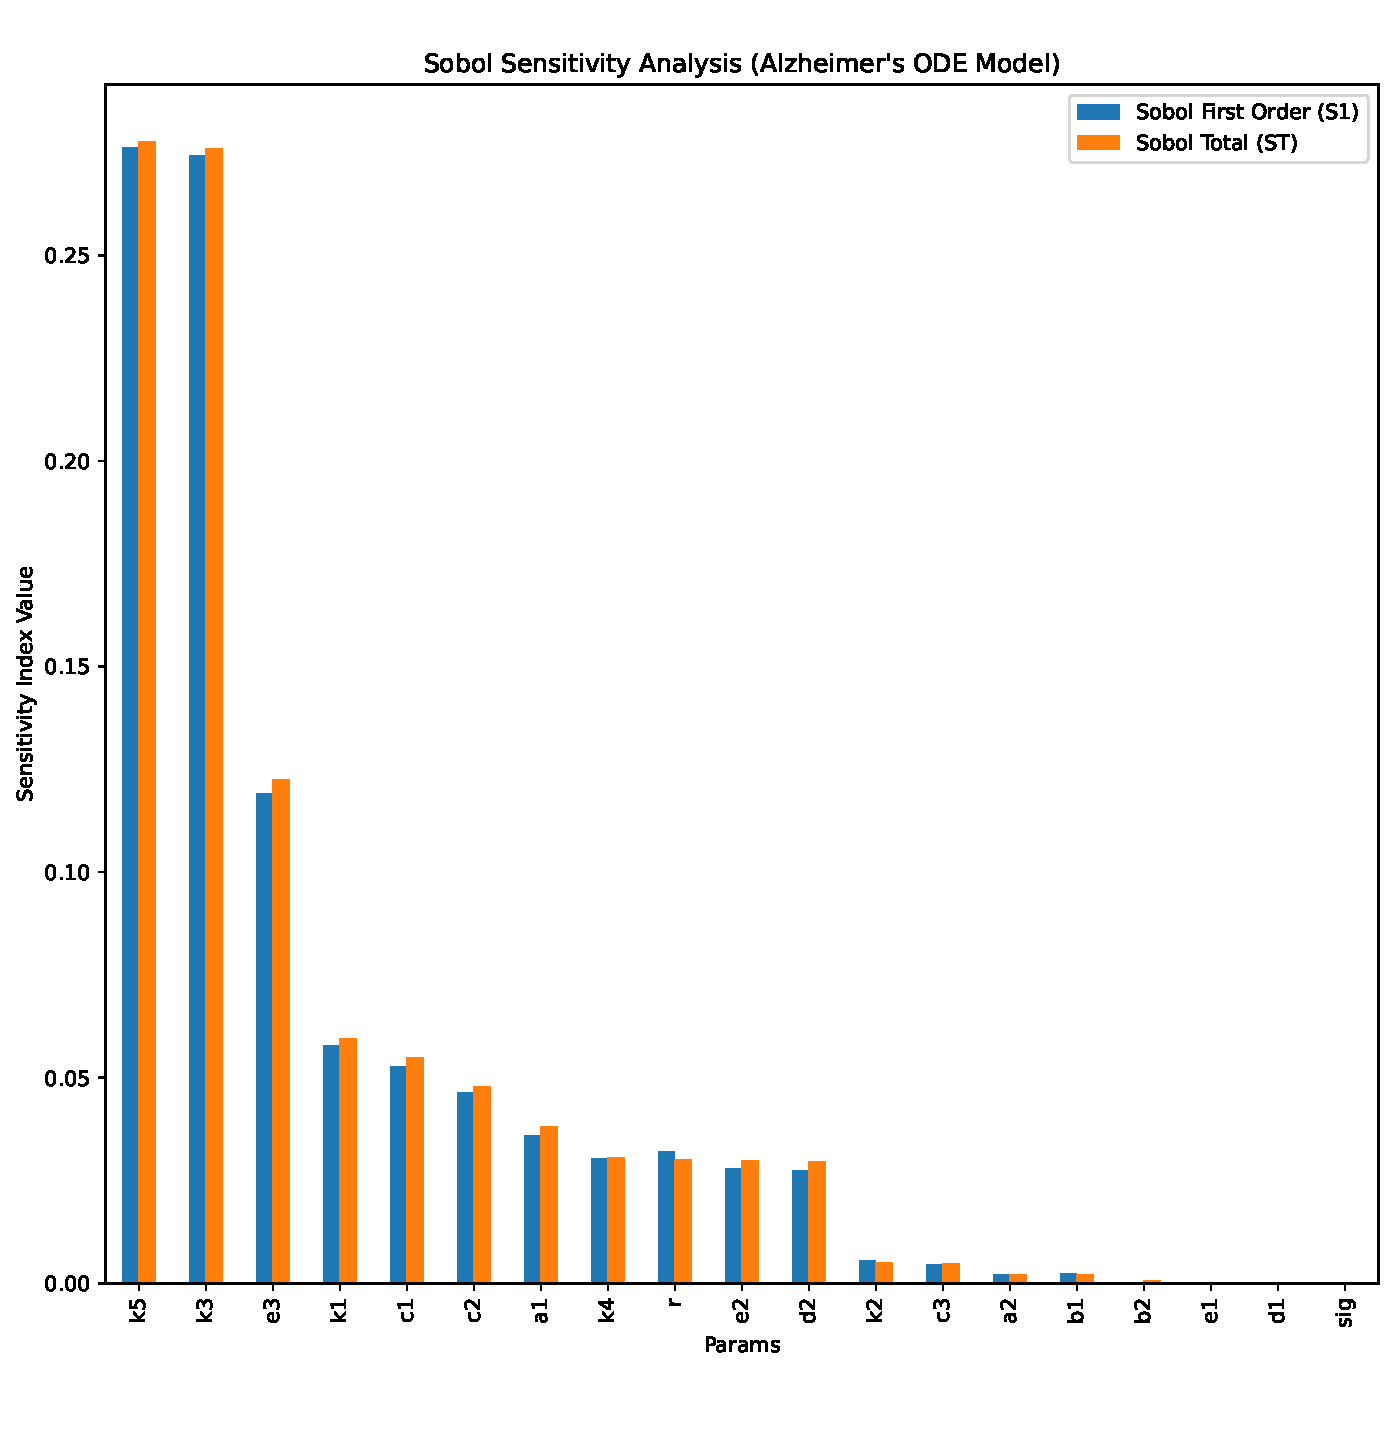
\includegraphics[width=0.4\textwidth]{img/sens_img_1.pdf}
        \caption{Visualization of sobol orders at $N=2^{10}$.}
        \label{fig:sensitivity-analysis}
    \end{figure}}

    \only<3>{\begin{figure}[htbp]
        \centering
        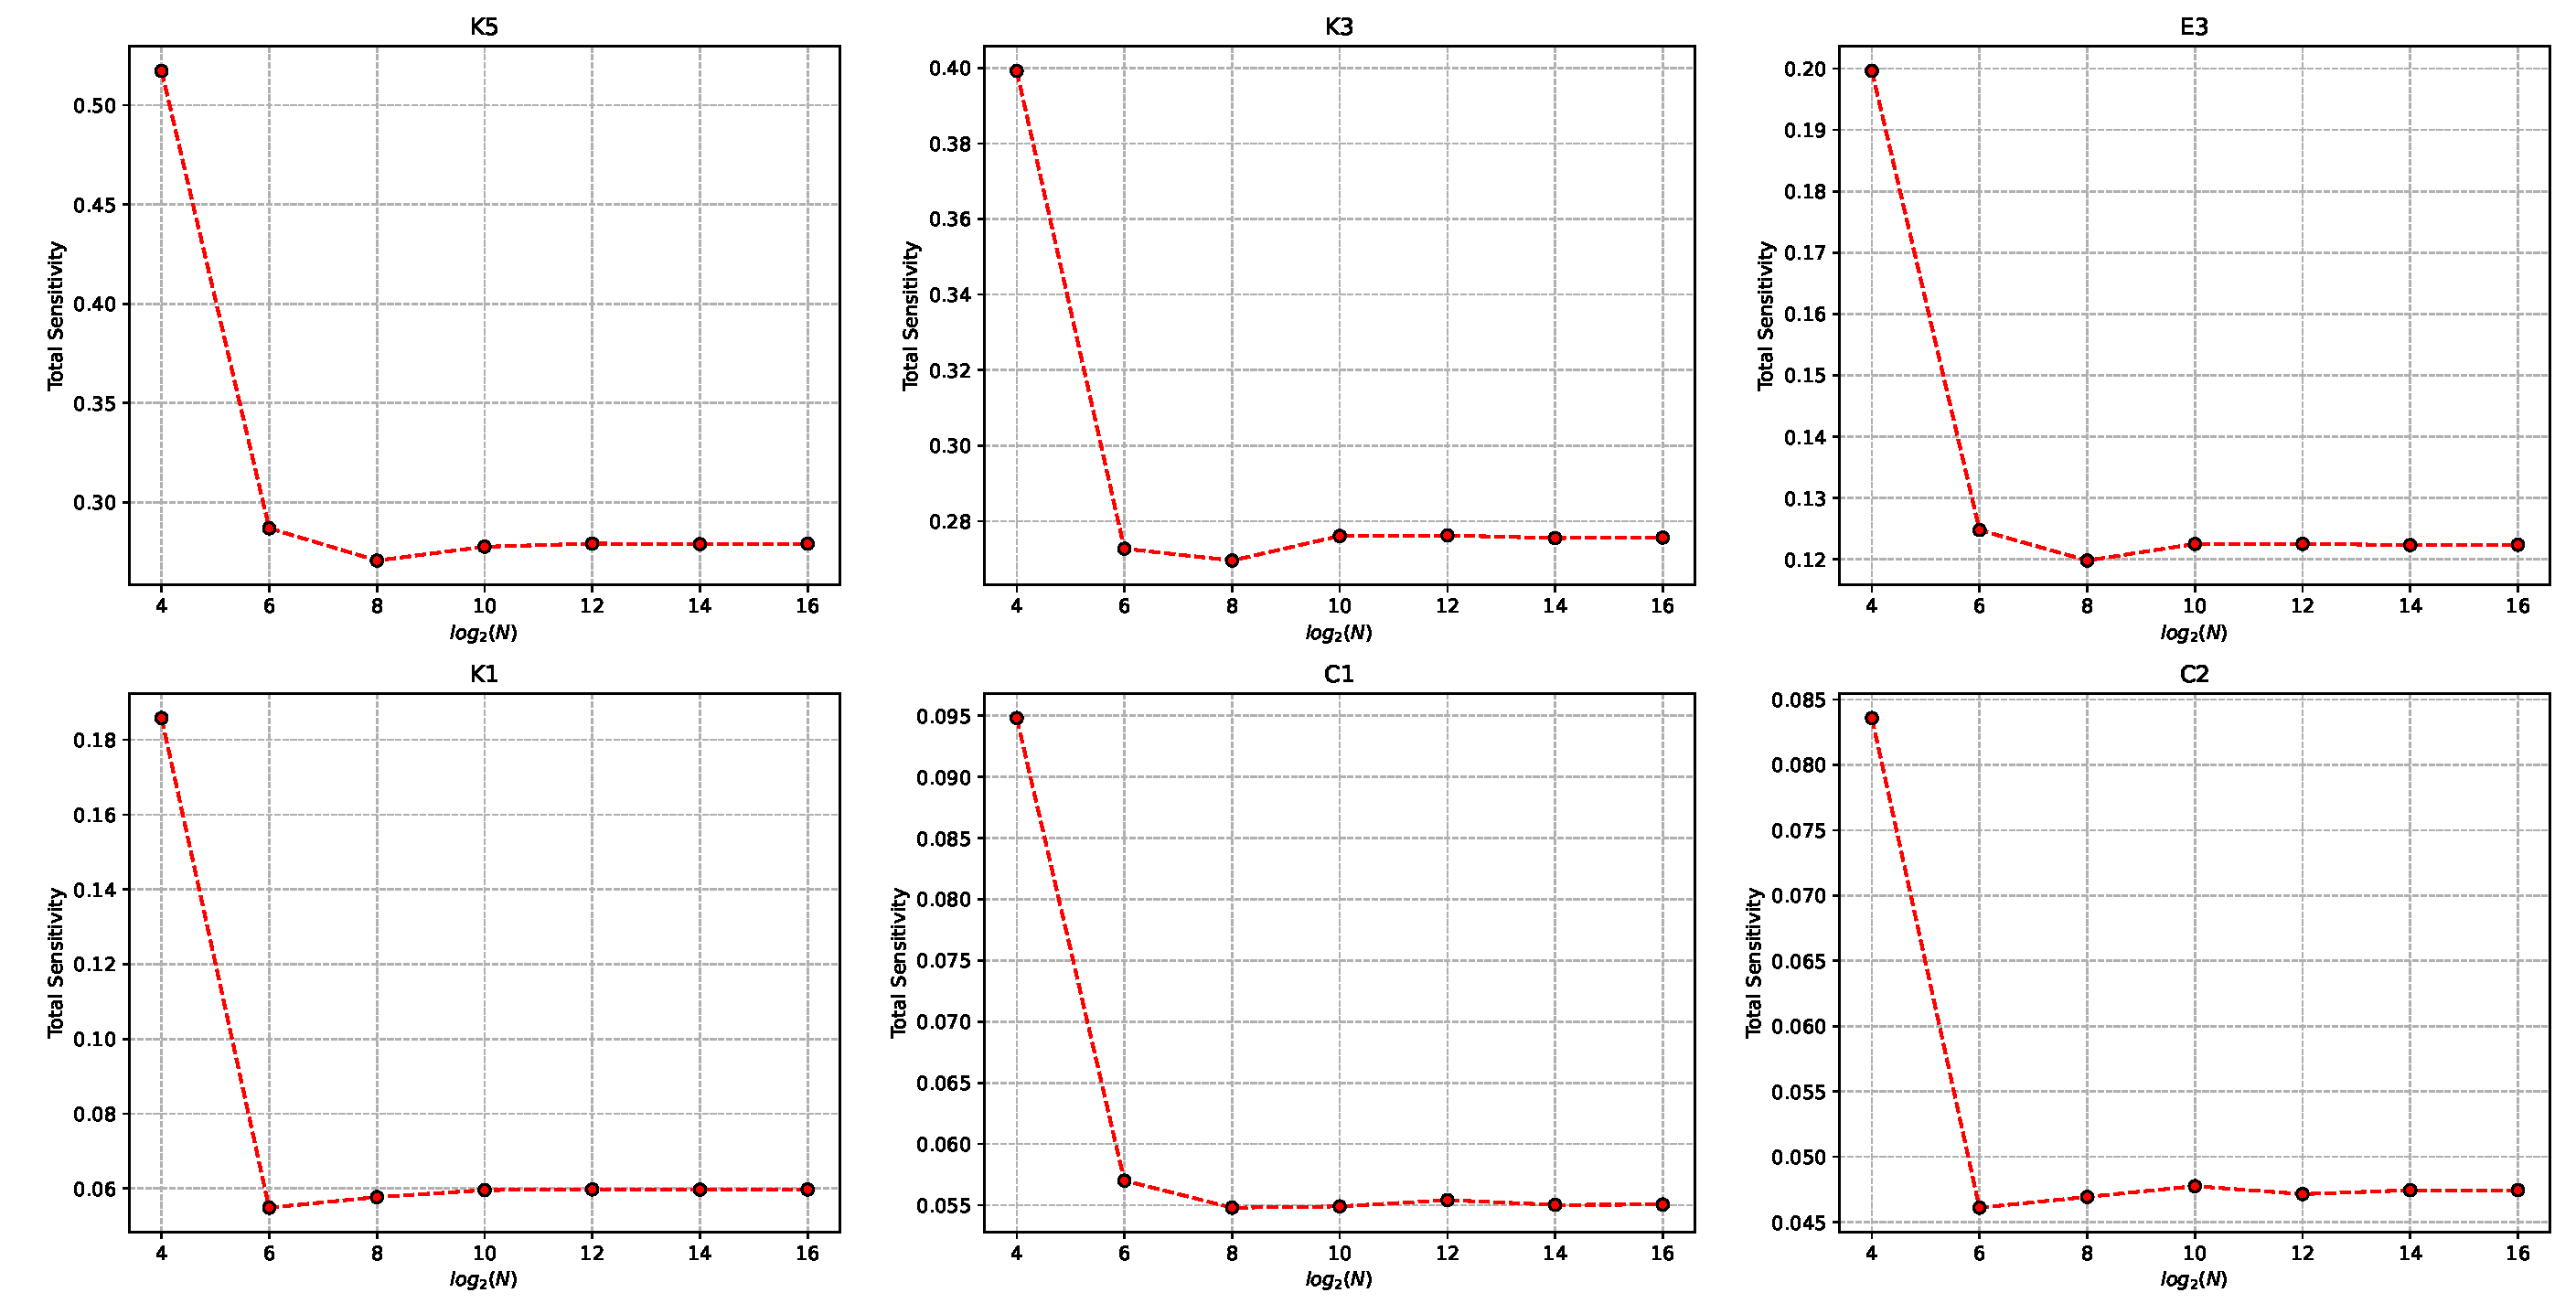
\includegraphics[width=0.8\textwidth]{img/6-most-sens-params.pdf}
        \caption{Six most sensitive parameters across $N \in [2^4, 2^{16}]$.}
    \end{figure}
    }
\end{frame}

\subsection{Optimal Control}
\begin{frame}
    Observing the model when a constant treatment for $A_\beta$, $Ca$, and $\tau$, it is suggested that treatments which lower calcium are not as relevant as initially assumed; rather, $\tau$ is the most important treatment avenue.
    \begin{figure}[htbp]
        \centering
        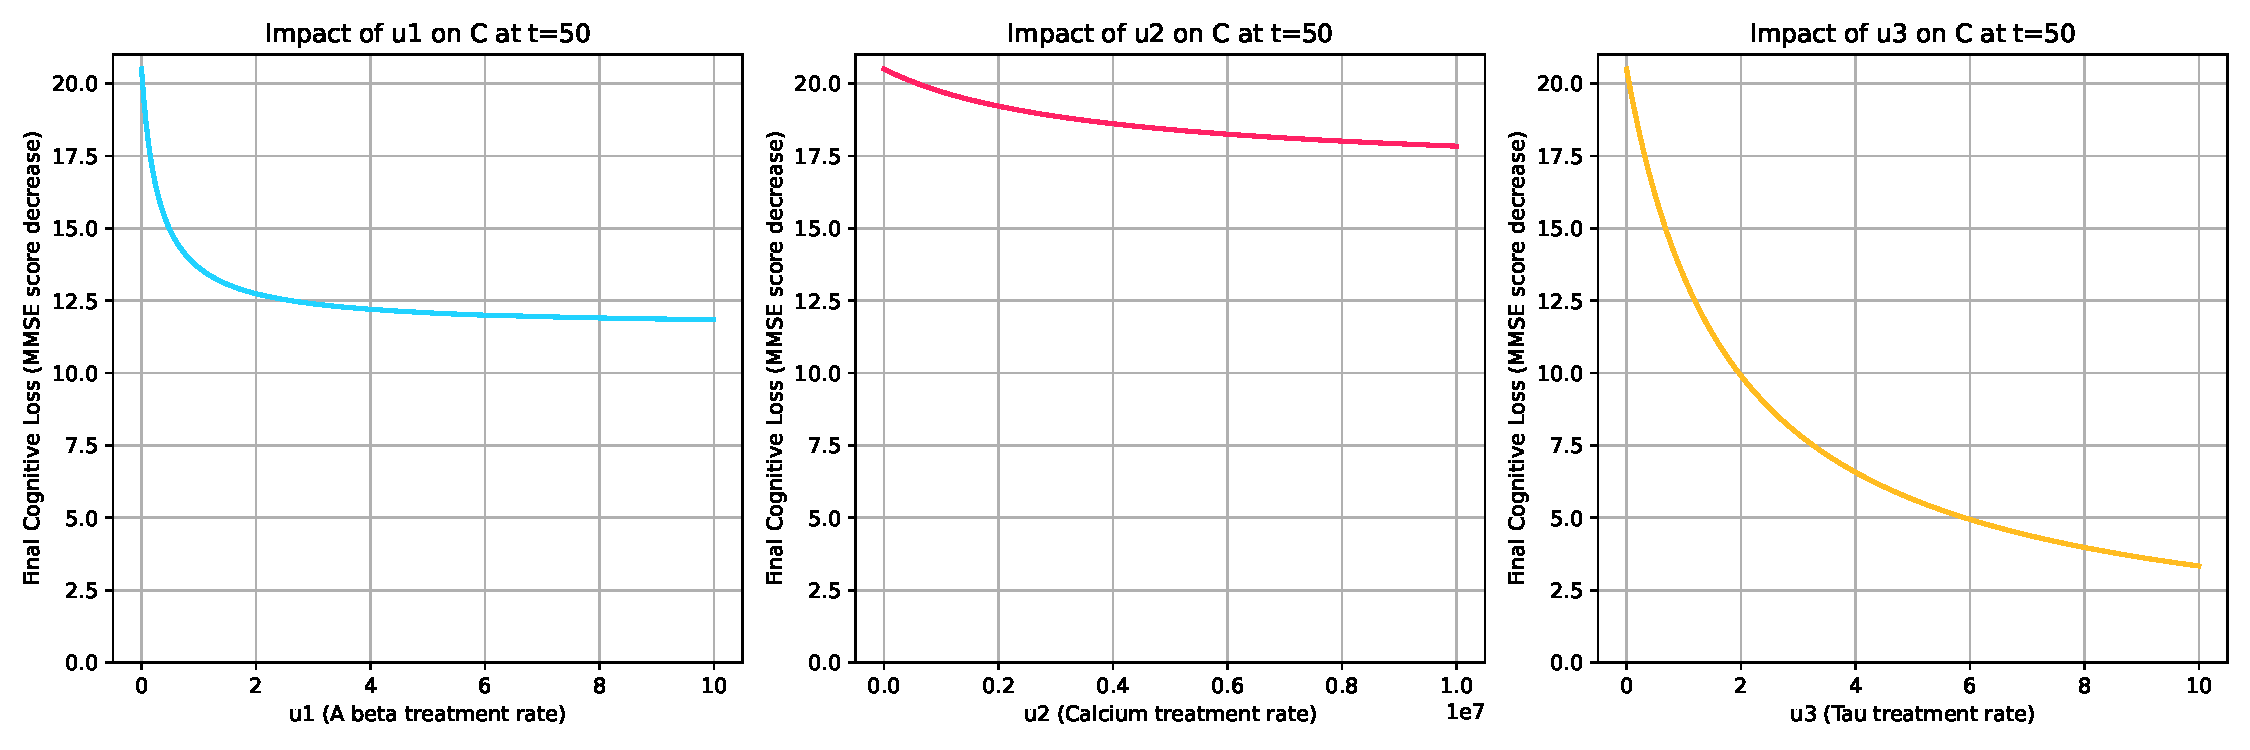
\includegraphics[width=0.8\textwidth]{img/alzgraph2.pdf}
        \caption{Constant treatments on $A_\beta$, Ca, and $\tau$.}
    \end{figure}
\end{frame}

\begin{frame}{Optimal Control}
    Recall the system of equations:
    \begin{align*}
        \frac{dA _{\beta}}{dt} &= a _{1} + a _{2}\frac{Ca }{Ca+\sigma} - k _{1}A _{\beta}-u _{1}A _{\beta}\\
        \frac{dCa}{dt} &= b _{1}+b _{2}A _{\beta}-k _{2}Ca - u _{2}Ca\\
        \frac{d \tau}{dt} &= c _{1}+c _{2}A _{\beta}+c _{3}Ca-k _{3}\tau-u _{3}\tau\\
        \frac{dN}{dt} &= d _{1}+d _{2}\tau-k _{4}N\\
        \frac{dC}{dt} &= e _{1}+e _{2}NR + e _{3}\tau-k _{5}C
    \end{align*}

    The purpose of optimal control is to determine the best way to administer treatments with minimal side effects (cost). The optimization problem is to minimize the objective function,
    \[J(u_1, u_2, u_3) = \int_0^K A_1 N + A_2 C + A_3 u_1^2 + A_4 u_2^2 + A_5 u_3^2 \, dt,\]

    where $u_n$ are non-negative treatment rates for each corresponding drug. In optimal control, each $u_n$ will be a function of time $u_n (t)$, so treatment levels can vary.
\end{frame}

\section{Concluding Remarks}
\begin{frame}{Future Directions}
    In order to provide a more interesting description of the mechanisms of AD, future directions include:
    \begin{itemize}
        \item Begin working with ADNI data in order to provide application modeled to real-world scenarios.
        \item Apply optimal control to simulations to find values for treatments.
    \end{itemize}
\end{frame}

\begin{frame}{References}
\printbibliography
\end{frame}

\begin{frame}{Acknowledgments}
    \begin{block}{}
        \begin{center}
            This work was supported primarily by the National Science Foundation EPSCoR Program under NSF Award OIA-2242812. We would also like to thank The Drs. Abernathy, as well as the Winthrop Mathematics Department, and The SURE Program for the opportunity to research.
        \end{center}
    \end{block}
\end{frame}

\begin{frame}{Closing}
    \begin{block}{}
       \centering Thank you. Questions?
    \end{block}
\end{frame}

\end{document}
